As mentioned before, the standard logistic model is inappropriate due to unsatisfied assumption of baseline of 1. It was fit to the same Ha Nam data using maximum likelihood with no accounting for censored titres (observations of 5 (below detectable) and 1280 (above detectable) were unchanged, all other observations were moved to the midpoint of the corresponding censored interval on a log scale). The fitted infection curve is in Figure \ref{lr-inf}.

\begin{figure}[htp]
	\centering
	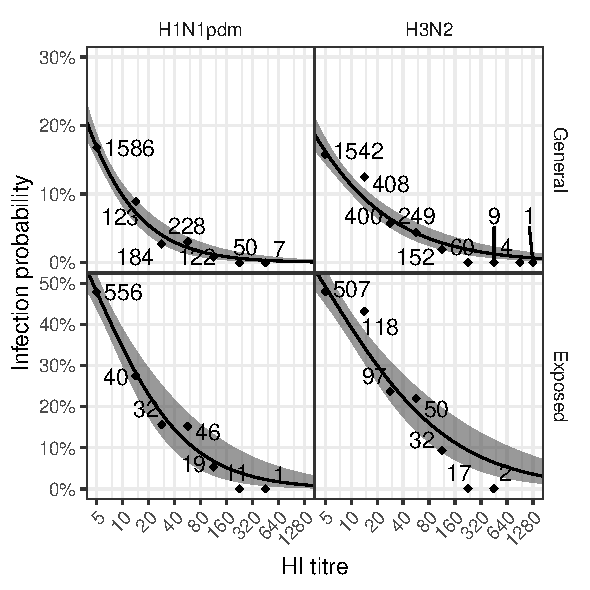
\includegraphics[width=0.8\textwidth]{../fit-logistic-plot/hanam-hi-inf.pdf}
	\caption{
		Fitted infection curves and confidence intervals from the standard logistic model fit to Ha Nam data (also shown in Figure \ref{HanamCounts}) using maximum likelihood with no accounting of censored titres (observations of 5 (below detectable) and 1280 (above detectable) were unchanged, all other observations were moved to the midpoints of the corresponding censored intervals on a log scale). The points are the infected proportions at the corresponding modified titre measurements (i.e. interval midpoints). The solid line is the point estimates. The shaded region is the 95\% confidence interval. The numbers next to the points are the total sample size of the corresponding groups.
	}
	\label{lr-inf}
\end{figure}

While the infection curves appear to fit the data well, it is problematic to generate a protection curve from these results. There are two options for the protection curve. One is to use the same procedure as was used in the scaled logit fit --- divide the fitted infection probabilities by the baseline (here assumed to be 1, so the fitted values would not change) and subtract the resulting relative-to-baseline infection probabilities from 1. The protection curves resulting from this procedure are in Figure \ref{lr-prot-abs}.

The other option for generating a protection curve is to calculate the fitted probability of infection at a give titre and divide that by the fitted probability of infection at the titre of 5 (or any other) thereby generating a curve that shows relative-to-5 infection probabilities (as opposed to relative-to-baseline). The variance of this quantity may be estimated by using the bootstrap method. Subtracting these relative-to-5 infection probabilities from 1 generates curves shown in Figure \ref{lr-prot-rel}.

\begin{figure}[htp]
	\centering
	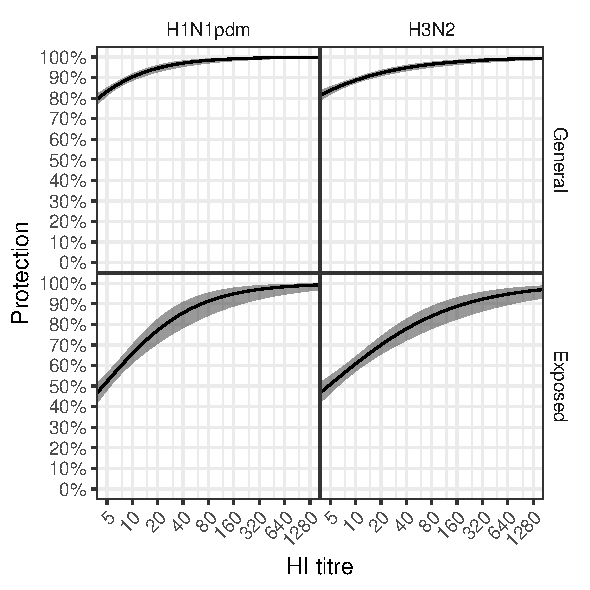
\includegraphics[width=0.8\textwidth]{../fit-logistic-plot/hanam-hi-prot.pdf}
	\caption{
		Fitted protection curves and confidence intervals from the standard logistic model fit to Ha Nam data (also shown in Figure \ref{HanamCounts}) using maximum likelihood with no accounting of censored titres (observations of 5 (below detectable) and 1280 (above detectable) were unchanged, all other observations were moved to the midpoints of the corresponding censored intervals on a log scale). The solid line is the point estimates. The shaded region is the 95\% confidence interval.
	}
	\label{lr-prot-abs}
\end{figure}

\begin{figure}[htp]
	\centering
	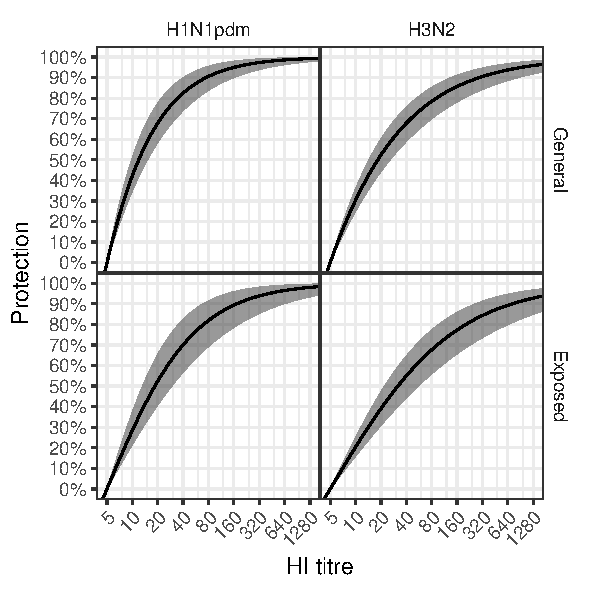
\includegraphics[width=0.8\textwidth]{../fit-logistic-boot-plot/hanam-hi-prot-rel.pdf}
	\caption{
		Fitted relative-to-5 protection curves and confidence intervals from the standard logistic model fit to Ha Nam data (also shown in Figure \ref{HanamCounts}) using maximum likelihood with no accounting of censored titres (observations of 5 (below detectable) and 1280 (above detectable) were unchanged, all other observations were moved to the midpoints of the corresponding censored intervals on a log scale). Solid lines are the point estimates, with shaded regions the 95\% confidence interval. The bounds for the confidence interval were obtained by using the bootstrap method (10,000 samples).
	}
	\label{lr-prot-rel}
\end{figure}

While the relative-to-5 protection curves (Figure \ref{lr-prot-rel}) appear more plausible than the relative-to-baseline protection curves (Figure \ref{lr-prot-abs}), both result from fitting a model with an unsatisfied assumption and neither method of generating protection curves from logistic regression model reliably produces accurate results. In addition, the high confidence in the results (small errors in Figures \ref{lr-prot-rel} and \ref{lr-prot-abs}) is misplaced as it is a result of a string assumption on the data that is unfounded.

The relative-to-5 curve (Figure \ref{lr-prot-rel}) presents an additional problem. The curve shows how much ``better'' different titres are at protecting against infection than the titre of 5.
There is nothing inherently special about this threshold of 5. Its choice is based on the lower dilution of 10 which is necessitated by the pre-treatment of sera. The curves may look substantially different if a different threshold (e.g. 10 or 1) is chosen. This hampers the interpretability and comparison of results.
